\chapter{Implementazione} %\label{1cap:spinta_laterale}
% [titolo ridotto se non ci dovesse stare] {titolo completo}
%

\begin{citazione}
Nell'ambito del presente capitolo verranno trattate le scelte effettuate per l'implementazione degli algoritmi facenti parte della \emph{pipeline} di compressione. Verrà posta particolare attenzione ai dettagli implementativi della \emph{sBWT} in quanto risulta essere l'algoritmo più pesante in termini di spazio occupato e di tempo impiegato. Verrà, successivamente, fornita una descrizione delle strategie impiegate per l'implementazione della \emph{bMTF} e della \emph{RLE}. Il capitolo si conclude con la descrizione della scelta dell'algoritmo di \emph{Variable Length Prefix Code} da utilizzare. 
\end{citazione}
\newpage

\section{Panoramica sullo sviluppo dell'algoritmo} 
La scelta del linguaggio di programmazione da utilizzare per l'implementazione dell'algoritmo di compressione sicuro è ricaduta su \emph{Python}. Tale scelta è stata guidata dalla ricerca di un linguaggio semplice e flessibile che consentisse di implementare in modo agevole e veloce gli algoritmi descritti soffermandosi sui dettagli rilevanti. Il codice sorgente dell'algoritmo sviluppato è reperibile al seguente link: https://github.com/vincenzo-emanuele/Progetto-Compressione-Dati. Come mostrato nella figura \ref{fig:project} il progetto è stato suddiviso in 4 \emph{packages}: \emph{Bwt, Mtf, PC e Rle}, ognuno dei quali contiene il codice sorgente del corrispondente algoritmo della \emph{pipeline}. L'implementazione delle \emph{pipeline} di compressione e di decompressione è demandato a due file che fungono da tester dell'algoritmo complessivo, denominati \emph{compressione.py} e \emph{decompressione.py}. La cartella \emph{TestFiles} contiene i file input utilizzati per testare l'algoritmo con i relativi file output prodotti dal processo di compressione.
\begin{figure}[h]
    \centering
    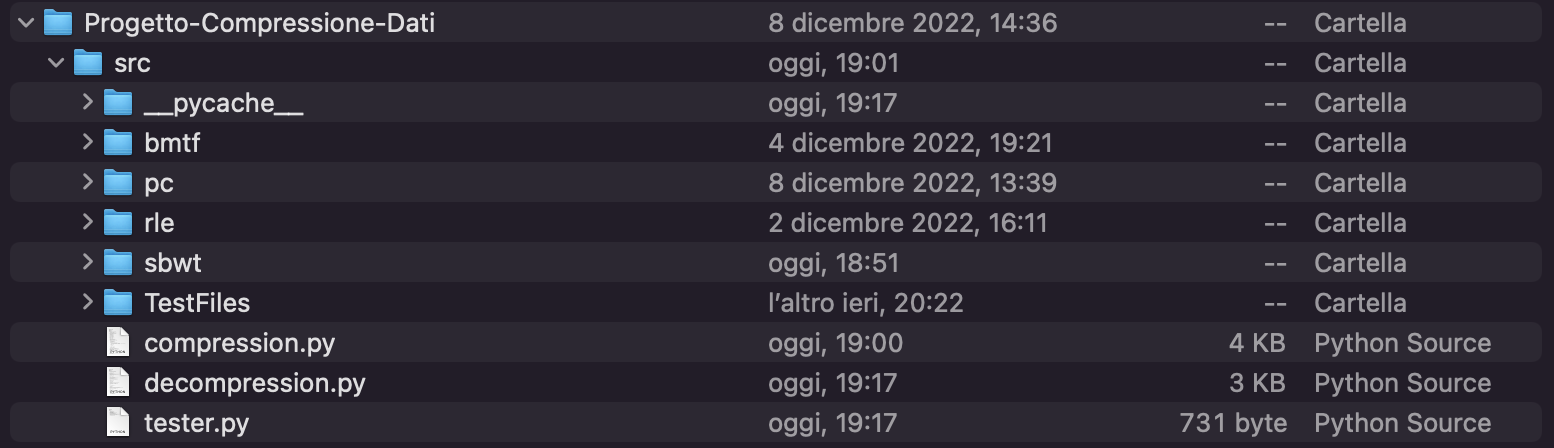
\includegraphics[width=1\textwidth]{Progetto Compressione Dati/capitoli/images/project.png}
\caption{Struttura del progetto}
    \label{fig:project}
\end{figure} \\
\section{Implementazione della sBWT} 
Implementare la \emph{sBWT} seguendo gli step dell'algoritmo non risulta conveniente in quanto la costruzione della matrice porterebbe ad un'esplosione della complessità in termini di tempo e di spazio. Per avere un'idea sulla complessità totale, basti pensare al fatto che la matrice da costruire contiene un numero di elementi pari al quadrato del numero di caratteri della stringa da comprimere; ciò significa che un file di appena 1MB porterebbe alla costruzione di una matrice di 1.099.511.627.776 elementi, occupando oltre 1TB di memoria. Per evitare tali situazioni è possibile applicare diverse ottimizzazioni che poggiano le proprie fondamenta sul fatto di lavorare sulla matrice senza costruirla esplicitamente, facendo uso di strutture ausiliarie costruite \emph{ad-hoc}. I paragrafi successivi descrivono nel dettaglio le ottimizzazioni attuate.
\subsection{Suffix Array}
Al fine di evitare la costruzione esplicita della matrice della \emph{BWT} sono stati utilizzati i \textbf{suffix array}, una struttura dati ben nota nell'ambito degli algoritmi. Formalmente, data una stringa $S$, il \emph{suffix array} $A$ di $S$ è un array di interi contenente le posizioni iniziali dei suffissi di $S$ in ordine lessicografico. Ad esempio, data la stringa $S=banana\$$ (\$ è il carattere speciale di \emph{EOF}), si indicizza la stringa come illustrato nella figura \ref{fig:sa1}.
\begin{figure}[h]
    \centering
    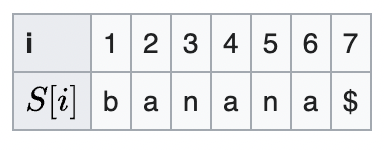
\includegraphics[scale=0.80]{Progetto Compressione Dati/capitoli/images/sa1.png}
\caption{Fonte: https://en.wikipedia.org/wiki/Suffix\_array}
    \label{fig:sa1}
\end{figure}\\
Successivamente si considerano tutti i suffissi: \{\emph{banana\$, anana\$, nana\$, ana\$, na\$, a\$, \$}\} e li si dispone in ordine lessicografico come illustrato nelle figure \ref{fig:sa2} e \ref{fig:sa3}.
\begin{figure}[h]
    \centering
    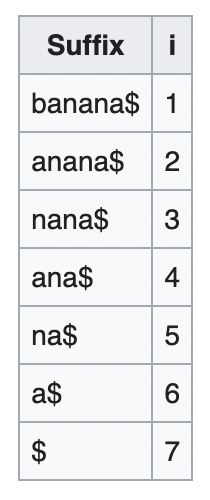
\includegraphics[scale=0.60]{Progetto Compressione Dati/capitoli/images/sa2.png}
\caption{Fonte: https://en.wikipedia.org/wiki/Suffix\_array}
    \label{fig:sa2}
\end{figure}
\begin{figure}[h]
    \centering
    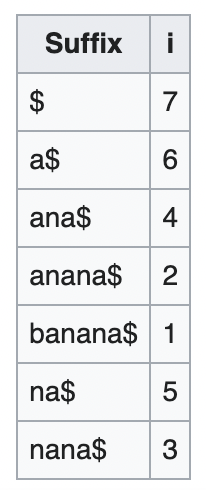
\includegraphics[scale=0.60]{Progetto Compressione Dati/capitoli/images/sa3.png}
\caption{Fonte: https://en.wikipedia.org/wiki/Suffix\_array}
    \label{fig:sa3}
\end{figure}\\
Il \emph{suffix array} risultante sarà $S=\{7, 6, 4, 2, 1, 5, 3\}$. Chiarito il funzionamento della struttura dati in questione, risulta utile descrivere il modo in cui la \emph{sBWT} la utilizza. La matrice $M$ utilizzata dalla \emph{sBWT} contiene, su ogni riga, tutti i suffissi di $S$ ordinati in ordine lessicografico. L'algoritmo computa, in primo luogo, il \emph{suffix array} $A$ relativo a $S$. Dal momento che tale \emph{array} contiene gli indici di tutti i suffissi di $S$ ordinati in ordine lessicografico, vi sarà una corrispondenza biunivoca tra le righe di $M$ e i suffissi "puntati" dagli indici di $A$. In particolare, la \emph{i-esima} riga di $M$ inizierà con il suffisso "puntato" dall'\emph{i-esimo} elemento di $A$. Risulta, dunque, immediato risalire all'ultimo carattere dell'\emph{i-esima} riga di $M$ in quanto sarà proprio l'\emph{i-1-esimo} carattere di $L$. \\ L'ottimizzazione appena descritta riduce la complessità spaziale della \emph{sBWT} da \emph{quadratica} a \emph{lineare}. La complessità temporale, invece, dipende dall'implementazione scelta per la costruzione dei \emph{suffix array}; nell'implementazione proposta dal presente lavoro è stata utilizzata un'implementazione avente complessità $\mathcal{O}(n\log^2{}n)$. Dal momento che la \emph{sBWT}, una volta aver ottenuto il \emph{suffix array}, computa il suo output in tempo $\mathcal{O}(n)$, l'algoritmo complessivo avrà complessità totale $\mathcal{O}(n\log^2{}n)$.
\subsection{Variante a blocchi}
\subsection{Parallelizzazione}
\subsection{Calcolo dell'inversa}
Il calcolo dell'inversa della trasformata è implementato evitando la costruzione esplicita della matrice al fine di scongiurare un'esplosione della complessità. Il paper \cite{burrows1994block} propone una strategia per il calcolo dell'inversa della \emph{BWT} che evita la costruzione della matrice. L'algoritmo prende in input il risultato $L$ della \emph{sBWT}, l'ordinamento lessicografico $O$ utilizzato in fase di compressione, fa uso di tre strutture ausiliarie denominate $C$, $P$ e $T$ e restituisce la stringa non compressa $S$:
\begin{itemize}
    \item $C$ è un dizionario costruito in modo tale che $C[ch]$ è il numero totale di istanze in $L$ dei caratteri che precedono $ch$ nell'ordinamento definito sull'alfabeto;
    \item $P$ è una lista costruita in modo tale che $P[i]$ è il numero di istanze del carattere $L[i]$ nel prefisso $L[0,\dots,i-1]$ di $L$;
\end{itemize}
Grazie a tali strutture, l'algoritmo riesce ad ottenere $S$. Le modalità mediante le quali tale stringa viene costruita si basano sul fatto che non sia necessario costruire esplicitamente una matrice per sfruttarne le proprietà. Dal momento che il funzionamento dell'algoritmo non risulta essere del tutto intuitivo, la sua trattazione verrà affrontata utilizzando come supporto un esempio pratico. Come illustrato nella figura \ref{fig:ibwt_ex} l'output restituito dalla \emph{BWT} sarà l'ultima colonna della matrice ordinata degli shift ciclici di $S$. Dal momento che il carattere di \emph{EOF} è il più piccolo secondo l'ordinamento lessicografico, la prima riga sarà sempre lo shift ciclico che come primo carattere ha l'\emph{EOF} seguito da $S$ (nel caso dell'esempio la riga $0$ della matrice è \emph{\$banana}). Ciò implica che l'ultimo carattere del testo da ricostruire (escludendo l'EOF) è il primo carattere di $L$, in questo caso $a$. Dal momento che per motivi di praticità l'output verrà ricostruito al contrario, il prossimo carattere da individuare è il predecessore di $a$ in $S$. Dato che si dispone solo della stringa $L$, è necessario individuare la riga che termina con il carattere $ch$ cercato in quanto corrisponderà esattamente all'indice di $L$ contenente $ch$; tale riga conterrà i caratteri della riga appena individuata \emph{shiftati} a destra di un carattere, dunque, comincerà con $a$. Sfruttando l'ordinamento della matrice è possibile accedere agevolmente alle righe che cominciano per $a$; a tale scopo risulta utile utilizzare la struttura $C$ in quanto $C[a]$ contiene il numero di occorrenze dei caratteri precedenti ad $a$ nell'ordinamento lessicografico presenti in $L$ (in questo caso $C[a]=1$). La riga $1$ di $M$ inizierà sicuramente per $a$, tuttavia la matrice potrebbe contenere più righe che cominciano con $a$, per cui è necessario stabilire quale di queste contenga come ultimo carattere il predecessore di $a$ cercato. Per fare ciò    
DA COMPLETARE
Conosciamo I = 0 perché visto che il \$ è più piccolo in ordine lessicografico la prima riga sarà sicuramente \$input (\$banana). Consideriamo L[I] che sarà l'ultima lettera della stringa da decodificare. A questo punto ci interessa trovare la riga che come ultima lettera ha la lettera che precede L[I] nel testo in chiaro (in questo caso a\$banan). Questa riga sarà proprio la riga I shiftata di uno a destra. Per trovare questa riga (che è una riga che comincia con L[i]) sfruttiamo il fatto che la matrice è ordinata. Come prima cosa ci spostiamo sulla prima riga che comincia con L[i]: per fare ciò sfruttiamo il vettore C che ci indica dove si trova. A questo punto dobbiamo capire quale tra le righe che cominciano per L[i] è quella che cerchiamo. Dal momento che abbiamo anche il vettore P, questo ci indica quale tra le righe è quella che ci interessa perché P conta il numero di occorrenze di L[I] nel prefisso letto fino a quel momento, dunque in base a quante volte abbiamo già incontrato L[i] sceglieremo la posizione giusta.
\section{Implementazione della bMTF} 
\section{Implementazione della RLE} 
\section{Scelta dell'algoritmo di PC} 
